\definecolor{gray75}{gray}{0.75}
\newcommand{\hsp}{\hspace{20pt}}
\titleformat{\chapter}[hang]{\Huge\bfseries}{\thechapter\hsp\textcolor{gray75}{|}\hsp}{0pt}{\Huge\bfseries}
\chapter{Introduction}


In this thesis, I present the methodology behind a statistical model I created, used to forecast the outcomes of and within\footnotemark{} Indian Premier League (IPL) Twenty20 (T20) cricket matches. I then test the performance of the model against two distinct benchmarks.

\footnotetext{I define the outcome of a match as simply, the team that wins the match (assuming it doesn’t finish in a tie, of course). In contrast, an outcome within a match includes answers to questions such as: which player scored the most runs? Who took the most wickets? Which team will score the most runs in the first six overs of their innings?}

Knowledge of the game of cricket, particularly the T20 format, is assumed throughout the report. If the reader is unfamiliar with how the game works, a short primer can be found in \autoref{chap: How Cricket Works}.

A second benchmark I test the model against will be historical odds from the sports betting market. I anticipate this to be a tougher test for the model to overcome, especially given the decently liquid markets\footnotemark{} for games in prized tournaments such as the IPL. Comparing against betting market data also has the added benefit of being able to test the model for performance in areas beyond simply match outcome. With this ball-by-ball modelling approach, almost every outcome in the match is simulated. These simulations can therefore be compared against what happened in the real world. Betting markets also tend to have offerings on many in-game propositions. These include: first over runs, batter to score the most runs, team to score the most sixes, etc. It will be interesting to check model performance in these areas, too.

\footnotetext{More liquidity tends to translate to high accuracy/efficiency of the market.}

\section{Motivation}

The motivation behind this project comes out of sheer curiosity to see whether this type of modelling could be effective in predicting the outcome of games. When considering the problem of modelling sports more generally, my first instinct is to think something like, ‘how can I best replicate this game artificially, from my computer?’ After having decided on the sport of cricket, it was obvious to me that a simulator of this kind mimics this game especially well. For example, one key factor in determining the outcome of a given delivery is the specific match-up between the batter and bowler. My knowledge of the game tells me that these match-ups can have a great deal of impact on the respective probabilities for each possible outcome of that ball. A ball-by-ball simulator here seems to account for these possible matchups very well, and better than any other approach I could think of. Before each delivery, the model will check to see who is the bowler, who is the batter, amongst other variables related to the state of the game at the time. Once these factors are known, it can sample from a distribution of probabilities, determined by these inputs. A more traditional modelling approach might take a more top-down stance. It may take team line-ups as an input and output some expected number of runs for each team across each innings as a whole. Where this approach falls short, in my opinion, is that it fails to attribute significant weight to the individual match-ups, central to the game. Moreover, in the format of T20, the outcome of each individual ball, has significantly more impact on the result of the match, compared with longer formats of the game. It therefore seems appropriate to try to model the game at the most granular level we can - that of the ball. 

\section{Overview of the Model}

The model that I propose can be broken down into several parts. The first is essentially a multi-class classification problem. Given there are only a finite number of possible outcomes that can happen from each ball, a probability can be assigned to each of these by the model, given a set of input parameters. A typical distribution based on frequentist probabilities across the dataset can be found below in \autoref{fig:my_label}. Incidentally, this is the exact distribution used in the naïve, benchmark model.

\begin{figure}
    \centering
    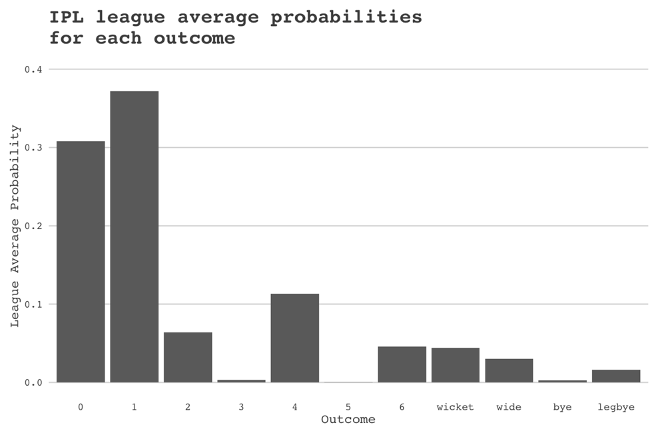
\includegraphics{images/Picture 1.png}
    \caption{Showing the probability distribution of the 11 possible outcomes from a delivery.}
    \label{fig:my_label}
\end{figure}

Based on which outcome gets sampled here, subsequent questions are asked, and the responses are sampled in a similarly probabilistic manner to above. For example, it is possible and not uncommon for a no-ball to be bowled by the bowler, in addition to the batsman scoring runs. This is why ‘no-ball’ is not one of the 11 initial outcomes. So if the outcome is one from zero to six runs, we sample to check for a no-ball. Runouts are also possible in addition to runs and byes (assuming no boundary is scored) so this is checked and sampled at the end of a ‘ball’ simulation. As we’ll discover in section 2, this practice of going beyond the initial sampling is a step beyond what has been done before in previous experiments of this kind.

Finally, the results of each delivery within a simulated game are stored in a dedicated R dataframe, while the results of each match of the entire series of simulations are stored in a separate dataframe. Based on the outcome of the prior ball, the simulator makes the necessary adjustments to the state of the game (e.g. batters switch ends if an odd number of runs are scored, bowler changes if the over has just ended, etc.) and we continue with the next delivery.
